\RequirePackage{fix-cm}
\documentclass[12pt,a4paper]{article}
\usepackage[utf8]{inputenc}
\usepackage[T1]{fontenc}
\usepackage{lmodern}
\usepackage[portuguese]{babel}
\usepackage{geometry}
\usepackage{graphicx}
\usepackage{amsmath}
\usepackage{booktabs}
\usepackage{hyperref}
\usepackage{natbib}
\usepackage{caption}
\usepackage{float}
\usepackage{setspace}
\usepackage{indentfirst}
\usepackage{fancyhdr}
\usepackage{titlesec}

\geometry{margin=2.5cm, top=2.5cm, bottom=2.5cm}
\onehalfspacing
\setlength{\parindent}{1.25cm}
\setlength{\parskip}{0.25em}
\setlength{\headheight}{15pt}

\hypersetup{
  colorlinks=true,
  linkcolor=black,
  citecolor=black,
  urlcolor=black
}

\pagestyle{fancy}
\fancyhf{}
\cfoot{Página \thepage}
\renewcommand{\headrulewidth}{0pt}

\titleformat{\section}
  {\normalfont\Large\bfseries}{\thesection}{1em}{}
\titleformat{\subsection}
  {\normalfont\large\bfseries}{\thesubsection}{1em}{}

\title{\textbf{Previsão da Variação Mensal dos Preços das Ações em França:\\
Uma Abordagem Comparativa com SARIMAX, VAR e MLP}}

\author{André Soares \and António Navalhas \and Lifan Chen \and Pedro Lourenço }
\date{}
\addto\captionsportuguese{\renewcommand{\contentsname}{Índice}}
\begin{document}

\pagenumbering{arabic}

\begin{titlepage}
  \thispagestyle{empty}
  \centering
  \vspace*{2.0cm}

  {\LARGE\bfseries Previsão da Variação Mensal dos Preços das Ações em França:\par}
  \vspace{0.35cm}
  {\Large Uma Abordagem Comparativa com SARIMAX, VAR e MLP\par}

  \vfill

  {\large
  André Soares, aluno n.º 98306\\[0.25cm]
  António Navalhas, aluno n.º 108187\\[0.25cm]
  Lifan Chen, aluno n.º 136520\\[0.25cm]
  Pedro Lourenço, aluno n.º 133931\par}

  \vfill

  {\large Mestrado: Ciência de Dados\par}
  \vspace{0.55cm}
  {\large Unidade curricular: Análise de Séries Temporais e Previsão\par}
  \vspace{0.55cm}
  {\large Docente: Diana Mendes\par}
  \vspace{0.55cm}
  {\large ISCTE -- Instituto Universitário de Lisboa\par}

  \vfill

  {\large Maio 2026\par}

  \vspace*{1.0cm}
\end{titlepage}

\clearpage
\tableofcontents
\clearpage

% =============================================================
\section{Introdução}
% =============================================================

O mercado acionista francês é um dos maiores da zona euro em termos de capitalização bolsista e funciona como barómetro da atividade económica europeia continental. A variação mensal do índice de preços das ações em França reflete não só expectativas sobre os lucros das empresas cotadas, mas também condições macroeconómicas mais gerais, em particular a incerteza de política económica e as flutuações cambiais que afetam a competitividade das empresas francesas.

A previsão de retornos acionistas é um problema central em finanças quantitativas. A hipótese dos mercados eficientes \citep{fama1970efficient} sugere que toda a informação pública é rapidamente incorporada nos preços, o que torna a previsão sistemática difícil. Ainda assim, existe evidência de alguma previsibilidade em horizontes curtos, sobretudo quando se incluem variáveis macroeconómicas como preditores \citep{baker2016measuring}. No caso francês, a economia é sensível ao ambiente regulatório europeu (BCE, Comissão Europeia) e às relações comerciais transatlânticas, o que justifica a inclusão de indicadores de incerteza política e de taxa de câmbio.

Neste trabalho comparam-se três modelos de famílias distintas: o SARIMAX \citep{box2015time}, que combina dinâmica autorregressiva com variáveis exógenas e sazonalidade; o VAR \citep{lutkepohl2005new}, que modela as relações entre várias séries ao mesmo tempo; e o MLP (\textit{Multilayer Perceptron}) \citep{haykin2009neural}, usado para testar a possibilidade de relações não-lineares entre desfasamentos e retornos futuros. Esta comparação permite perceber se uma abordagem linear com variáveis exógenas, um modelo multivariado ou um modelo não-linear se ajusta melhor ao problema em estudo.

São usadas três séries da FRED: (i)~SPASTT01FRM657N, a variação percentual mensal do índice de ações francês; (ii)~FREUINDXM, o índice de incerteza de política económica para França (EPU), desenvolvido por \citet{baker2016measuring}; e (iii)~DEXUSEU, a taxa de câmbio EUR/USD. A escolha do EPU francês, em vez de um índice global, permite aproximar melhor a incerteza sentida no contexto doméstico, por exemplo em períodos de eleições, reformas laborais ou discussão de política fiscal.

Formulam-se três questões de investigação:

\begin{itemize}
  \item[\textbf{Q1}] A incerteza económica (EPU) e a taxa de câmbio (EUR/USD) contribuem estatisticamente para a previsão da variação mensal do índice de ações francês?
  \item[\textbf{Q2}] Qual dos três modelos, SARIMAX, VAR e MLP, apresenta melhor desempenho preditivo fora da amostra?
  \item[\textbf{Q3}] Qual a trajectória prevista para os dez meses seguintes ao final da amostra (maio de 2026 a fevereiro de 2027)?
\end{itemize}

Os dados cobrem janeiro de 1999 a abril de 2026 (328~obs.), englobando crises relevantes para o contexto francês: o \textit{dot-com crash} (2001), a crise financeira global (2008), a crise da dívida soberana europeia (2011--12), os \textit{Gilets jaunes} (2018--19) e o COVID-19 (2020).

% =============================================================
\section{Background}
% =============================================================

\subsection{SARIMAX}

O ARIMA$(p,d,q)$ modela uma série como função linear de $p$~valores passados (AR) e $q$~erros passados (MA), após $d$~diferenciações para estacionariedade \citep{box2015time}. A componente AR capta a persistência da série; no caso de retornos mensais, isto pode corresponder a algum \textit{momentum} de curto prazo. A componente MA representa choques transitórios, como um acontecimento pontual que afeta o índice num mês, mas cujo efeito se dissipa nos meses seguintes. A extensão SARIMA acrescenta termos sazonais com periodicidade $s{=}12$, permitindo testar padrões associados ao calendário.

O SARIMAX inclui variáveis exógenas:
\begin{equation}
y_t = \beta^\top x_t + \phi(B)\,\Phi(B^s)\,(1{-}B)^d(1{-}B^s)^D\,\varepsilon_t
\end{equation}
onde $x_t$ contém EPU e EUR/USD transformados. O coeficiente $\beta$ mede o efeito contemporâneo destas variáveis sobre o retorno, controlando pela dinâmica autorregressiva. No contexto francês, espera-se $\beta_{\text{EPU}} < 0$: incerteza política elevada (e.g., eleições disputadas, reformas das pensões) deprime os retornos.

\subsection{VAR}

O VAR$(k)$ é um sistema de $n$~equações simultâneas \citep{lutkepohl2005new}:
\begin{equation}
y_t = A_1 y_{t-1} + \cdots + A_k y_{t-k} + \varepsilon_t
\end{equation}
onde $y_t$ é um vetor ($n{=}3$: Stocks, EPU, EUR/USD). A principal vantagem face ao SARIMAX é tratar todas as variáveis como potencialmente endógenas. Assim, o modelo pode captar não só o efeito do EPU e do câmbio sobre o índice acionista, mas também o movimento inverso, por exemplo quando quedas no mercado aumentam a incerteza medida nos meses seguintes. A seleção de $k$ pelo AIC procura equilibrar capacidade de ajuste e parcimónia. Os resíduos são depois avaliados com o teste de Ljung-Box, para verificar se ainda existe autocorrelação relevante.

\subsection{MLP}

O MLP é uma rede \textit{feedforward} com camadas ocultas e ativações não-lineares (ReLU: $f(z){=}\max(0,z)$; tanh) \citep{haykin2009neural}. A sua inclusão no trabalho justifica-se pela possibilidade de captar interações não-lineares entre variáveis. Por exemplo, o impacto do EPU nos retornos pode não ser simétrico: períodos de incerteza elevada podem penalizar mais o mercado do que períodos de baixa incerteza o beneficiam. Ainda assim, com cerca de 290 observações de treino e 18 variáveis de entrada, existe risco de sobreajustamento, pelo que se usam normalização, \textit{early stopping} e validação cruzada temporal.

% =============================================================
\section{Modelos}
% =============================================================

\paragraph{SARIMAX.} \mbox{}\\ A ordem $(p,d,q)(P,D,Q)_{12}$ é selecionada com \texttt{auto\_arima} (\texttt{pmdarima}), usando o critério AIC e limites de pesquisa $p,q \leq 4$ e $P,Q \leq 2$. As variáveis exógenas são $\Delta\log(\text{EPU}_t)$ e $\Delta\log(\text{EUR/USD}_t)$. Esta transformação em diferença logarítmica permite trabalhar com taxas de variação e melhora a estacionariedade das séries. Na previsão fora da amostra usam-se os valores observados das exógenas (\textit{ex-post}); na previsão a 10~meses estas variáveis são mantidas na sua média histórica, representando um cenário neutro. A estimação é feita por máxima verossimilhança gaussiana e o diagnóstico inclui autocorrelograma dos resíduos, Q-Q plot e teste de heterocedasticidade.

\paragraph{VAR.} \mbox{}\\ O VAR é estimado como um sistema trivariado com Stocks, $\Delta\log\text{EPU}$ e $\Delta\log\text{EUR/USD}$. O número de desfasamentos é selecionado pelo AIC ($k = 1, \ldots, 12$). Os resíduos são verificados com o teste de Ljung-Box ao lag~12. A previsão é recursiva, ou seja, cada passo usa as previsões anteriores como input. A causalidade de Granger é avaliada dentro deste sistema.

\paragraph{MLP.} \mbox{}\\ Entrada: 18~neurónios ($6\text{ lags} \times 3\text{ séries}$). Camadas ocultas: \textit{grid search} entre $(50)$, $(100)$, $(50{,}25)$, $(100{,}50)$. Activação: ReLU ou tanh. Taxas: $\{0{,}001;\,0{,}01\}$. Saída: 1~neurónio linear. Perda: MSE. Normalização: \texttt{StandardScaler} ($\mu{=}0$, $\sigma{=}1$). \textit{Early stopping} com 15\% de validação. Selecção por 5~\textit{folds} temporais (\texttt{TimeSeriesSplit}). Previsão multi-passo: iterativa (output de $t{+}1$ alimenta $t{+}2$).

% =============================================================
\section{Experiências}
% =============================================================

\subsection{Dados e pré-processamento}

As três séries foram obtidas da FRED e cobrem janeiro de 1999 a abril de 2026 (328~obs. mensais após \textit{inner join}). A série Stocks é expressa em variação percentual e estacionária por construção. O EPU francês é publicado como índice em nível (base 100 = média histórica); o EUR/USD é uma taxa de câmbio em nível. Ambas são integradas de ordem~1, confirmado por ADF ($p > 0{,}05$ em nível). A transformação $\Delta\log(x_t)$ produz taxas de variação mensal estacionárias, verificadas por ADF ($p < 0{,}05$), Phillips-Perron ($p < 0{,}05$) e KPSS (não rejeição de $H_0$: estacionariedade).

A amostra inclui eventos com impacto significativo no mercado francês: a bolha tecnológica (CAC~40 perdeu 65\% em 2001--03), a falência do Lehman Brothers (queda de 13\% em outubro de 2008), a crise do euro (spreads soberanos franceses atingiram 200~b.p.\ em 2011), os protestos dos \textit{Gilets jaunes} (EPU francês atingiu picos históricos em 2018--19), e o COVID-19 (queda de 17\% em março de 2020). Esta diversidade de regimes torna a amostra adequada para testar a robustez dos modelos.

\subsection{Divisão temporal e avaliação}

A divisão da amostra é cronológica, com 90\% das observações para treino e 10\% para teste. O conjunto de treino contém 294 observações (fevereiro de 1999 a julho de 2023) e o conjunto de teste contém 32 observações (agosto de 2023 a abril de 2026). Este período final inclui a incerteza associada às eleições legislativas francesas de 2024 e a volatilidade geopolítica ligada ao conflito Rússia-Ucrânia, pelo que é uma janela exigente para avaliar previsões fora da amostra.

O SARIMAX é estimado no treino; a previsão no teste usa exógenas reais (\textit{ex-post}). O VAR prevê recursivamente. O MLP usa \texttt{GridSearchCV} (16~configs $\times$ 5~folds = 80~ajustes). A previsão a 10~meses (maio de 2026 a fevereiro de 2027) re-estima cada modelo com toda a amostra (326~obs.\ transformadas).

As métricas usadas são MAE, RMSE e MAPE. O RMSE é usado como critério principal por penalizar mais os erros grandes; o MAE dá uma leitura mais direta do erro médio; e o MAPE é reportado por comparabilidade, embora seja menos estável quando os retornos observados estão próximos de zero.

% =============================================================
\section{Resultados e Análise}
% =============================================================

De forma geral, os resultados mostram que o SARIMAX obtém o menor RMSE (3,13), o VAR o menor MAE (2,49), e o MLP fica em terceiro lugar. A incerteza económica é significativa contemporaneamente no SARIMAX. As previsões a 10 meses convergem para zero, consistente com a reversão para a média.

\subsection*{Q1: Contribuição das variáveis exógenas}

Os testes de causalidade de Granger (até 6~lags) mostram um padrão assimétrico. Nem o EPU nem o EUR/USD parecem antecipar os Stocks de forma estatisticamente significativa (EPU$\to$Stocks: $p=0{,}575$; EUR/USD$\to$Stocks: $p=0{,}773$). Já no sentido inverso há evidência estatística: Stocks$\to$EPU ($p=0{,}012$) e Stocks$\to$EUR/USD ($p=0{,}003$).

Uma leitura plausível é que o mercado acionista reage rapidamente a expectativas e notícias, antes de estas aparecerem de forma clara nos indicadores de incerteza \citep{fama1970efficient}. Assim, quedas no índice francês podem ser seguidas por maior cobertura mediática negativa e por um aumento do EPU. Um raciocínio semelhante pode explicar a relação com o EUR/USD, dado que períodos de maior aversão ao risco tendem a afetar também o mercado cambial.

Apesar de o EPU não apresentar precedência temporal sobre os Stocks nos testes de Granger, o seu coeficiente no SARIMAX é significativo ($p < 0{,}05$) e tem sinal negativo. Isto sugere uma relação contemporânea: em meses de maior incerteza, como no período da dissolução da Assembleia Nacional em junho de 2024, os retornos tendem a ser mais baixos. O VAR acrescenta outra peça a esta leitura, ao mostrar que choques nos retornos podem propagar-se para o EPU nos meses seguintes.

Assim, as variáveis exógenas parecem contribuir sobretudo por efeito contemporâneo e por dinâmicas cruzadas do sistema, e não tanto por anteciparem diretamente os retornos do índice.

\subsection*{Q2: Comparação do desempenho}

\begin{table}[H]
\centering\small
\caption{Métricas de previsão no conjunto de teste (32~obs.).}
\label{tab:metrics}
\begin{tabular}{lccc}
\toprule
\textbf{Modelo} & \textbf{MAE} & \textbf{RMSE} & \textbf{MAPE} \\
\midrule
SARIMAX & 2,54 & \textbf{3,13} & 260\% \\
VAR     & \textbf{2,49} & 3,22 & \textbf{158\%} \\
MLP     & 2,67 & 3,45 & 285\% \\
\bottomrule
\end{tabular}
\end{table}

O SARIMAX apresenta o menor RMSE (3,13), o que indica melhor desempenho quando se penalizam mais os erros grandes. O VAR, por outro lado, tem o menor MAE (2,49) e o menor MAPE (158\%), sugerindo previsões ligeiramente mais estáveis em termos médios. A diferença entre SARIMAX e VAR é pequena ($\Delta$RMSE $= 0{,}09$), pelo que a vantagem do SARIMAX deve ser interpretada com alguma cautela. Ainda assim, faz sentido que este modelo beneficie da informação contemporânea do EPU, sobretudo em meses de maior volatilidade.

O MLP fica em terceiro lugar ($\text{RMSE} = 3{,}45$). Este resultado não é surpreendente. A amostra de treino tem cerca de 290 observações, pouco para uma rede com 18 variáveis de entrada. Além disso, em séries financeiras mensais, o sinal preditivo tende a ser fraco face ao ruído. A previsão iterativa também contribui para este desempenho, porque erros pequenos nos primeiros passos podem acumular-se nos meses seguintes \citep{atsalakis2009surveying}.

O RMSE, entre aproximadamente 3,1 e 3,5 pontos percentuais, representa cerca de 70\% do desvio-padrão histórico da série ($\sigma \approx 4{,}5\%$). Ou seja, os modelos conseguem reduzir parte da incerteza, mas continuam longe de produzir previsões muito precisas, o que é normal em retornos financeiros mensais \citep{fama1970efficient}. Os valores de MAPE devem ser lidos com cuidado, pois ficam inflacionados quando o retorno observado está perto de zero.

No conjunto, o SARIMAX é o melhor modelo segundo o RMSE, enquanto o VAR é competitivo e até superior em MAE e MAPE. O MLP não consegue superar os modelos lineares nesta amostra.

\subsection*{Q3: Previsão a 10 meses}

Os três modelos, re-estimados com toda a amostra, preveem variações mensais de pequena amplitude ($<$2\% em absoluto). O VAR acumula $\approx$5\% de retorno em 10~meses, o MLP $\approx$3\%, e o SARIMAX $\approx$1\% (Figura~A2, apêndice). A convergência para zero reflete a estacionariedade da série: na ausência de choques, os modelos projetam os retornos para perto da média incondicional ($\approx$0,5\%/mês).

Em termos económicos, as previsões apontam para um mercado sem tendência forte no horizonte de maio de 2026 a fevereiro de 2027, com oscilações dentro de valores habituais para a série. O VAR é o modelo mais otimista, em parte porque incorpora a dinâmica conjunta entre as três variáveis e projeta um cenário relativamente estável para o EPU e para o EUR/USD.

Assim, a previsão a 10 meses sugere um mercado relativamente lateralizado, com retornos acumulados entre cerca de 1\% e 5\%, dependendo do modelo considerado.

% =============================================================
\section{Conclusão}
% =============================================================

O SARIMAX obteve o menor RMSE na previsão da variação mensal do mercado francês, confirmando a adequação de modelos lineares com exógenas para séries financeiras de frequência mensal. O VAR produziu desempenho competitivo e revelou dinâmicas cruzadas economicamente interpretáveis. O MLP não superou os modelos lineares, resultado expectável dada a dimensão da amostra e a natureza ruidosa dos retornos.

O resultado mais relevante para a literatura é a assimetria na causalidade de Granger: o mercado francês antecipa variações futuras da incerteza política e do câmbio, mas não é previsível a partir destes indicadores com desfasamento. Isto reforça a noção de eficiência semi-forte e sugere que a utilidade do EPU no SARIMAX reside no efeito contemporâneo, não na precedência temporal.

Como trabalho futuro: (i)~modelos híbridos ARIMA-MLP combinando interpretabilidade e flexibilidade; (ii)~redes LSTM para dependências de longo prazo; (iii)~variáveis de sentimento extraídas de notícias francesas (\textit{Le Monde}, \textit{Les Echos}) como substituto do EPU.

% =============================================================
% Referências
% =============================================================
\newpage
\phantomsection
\addcontentsline{toc}{section}{Referências}
\begingroup
\small
\bibliographystyle{plainnat}
\begin{thebibliography}{9}

\bibitem[Atsalakis \& Valavanis(2009)]{atsalakis2009surveying}
Atsalakis, G.S., \& Valavanis, K.P. (2009).
Surveying stock market forecasting techniques -- Part II: Soft computing methods.
\textit{Expert Systems with Applications}, 36(3), 5932--5941.

\bibitem[Baker et~al.(2016)]{baker2016measuring}
Baker, S.R., Bloom, N., \& Davis, S.J. (2016).
Measuring economic policy uncertainty.
\textit{The Quarterly Journal of Economics}, 131(4), 1593--1636.

\bibitem[Box et~al.(2015)]{box2015time}
Box, G.E.P., Jenkins, G.M., Reinsel, G.C., \& Ljung, G.M. (2015).
\textit{Time Series Analysis: Forecasting and Control}. 5.\textordfeminine~ed. Wiley.

\bibitem[Fama(1970)]{fama1970efficient}
Fama, E.F. (1970).
Efficient capital markets: A review of theory and empirical work.
\textit{The Journal of Finance}, 25(2), 383--417.

\bibitem[Haykin(2009)]{haykin2009neural}
Haykin, S. (2009).
\textit{Neural Networks and Learning Machines}. 3.\textordfeminine~ed. Pearson.

\bibitem[L\"{u}tkepohl(2005)]{lutkepohl2005new}
L\"{u}tkepohl, H. (2005).
\textit{New Introduction to Multiple Time Series Analysis}. Springer.

\end{thebibliography}
\endgroup

% =============================================================
% Apêndice
% =============================================================
\newpage
\appendix
\section{Figuras complementares}

\begin{figure}[H]
\centering
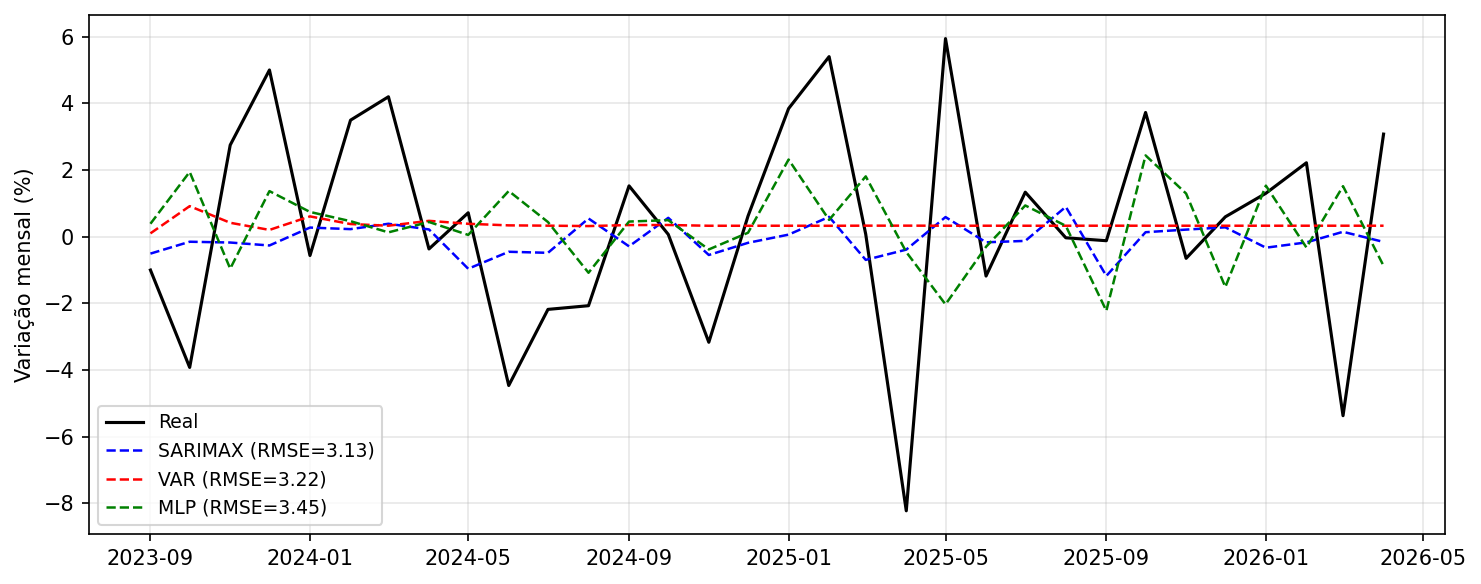
\includegraphics[width=\linewidth]{figures/comparison.png}
\caption{Figura A1: previsão fora da amostra, série real vs.\ os três modelos (agosto de 2023 a abril de 2026).}
\end{figure}

\begin{figure}[H]
\centering
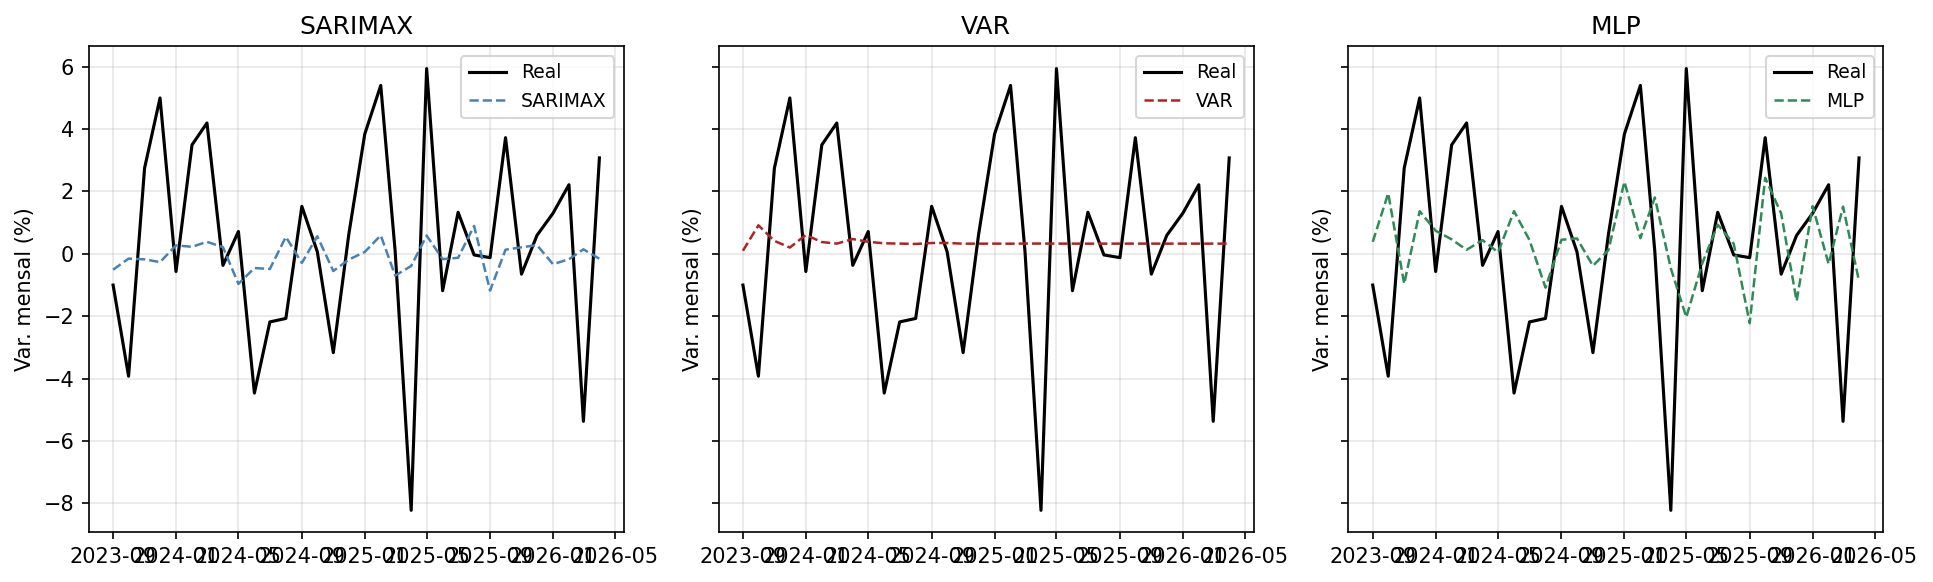
\includegraphics[width=\linewidth]{figures/individual.png}
\caption{Previsões individuais de cada modelo no conjunto de teste.}
\end{figure}

\begin{figure}[H]
\centering
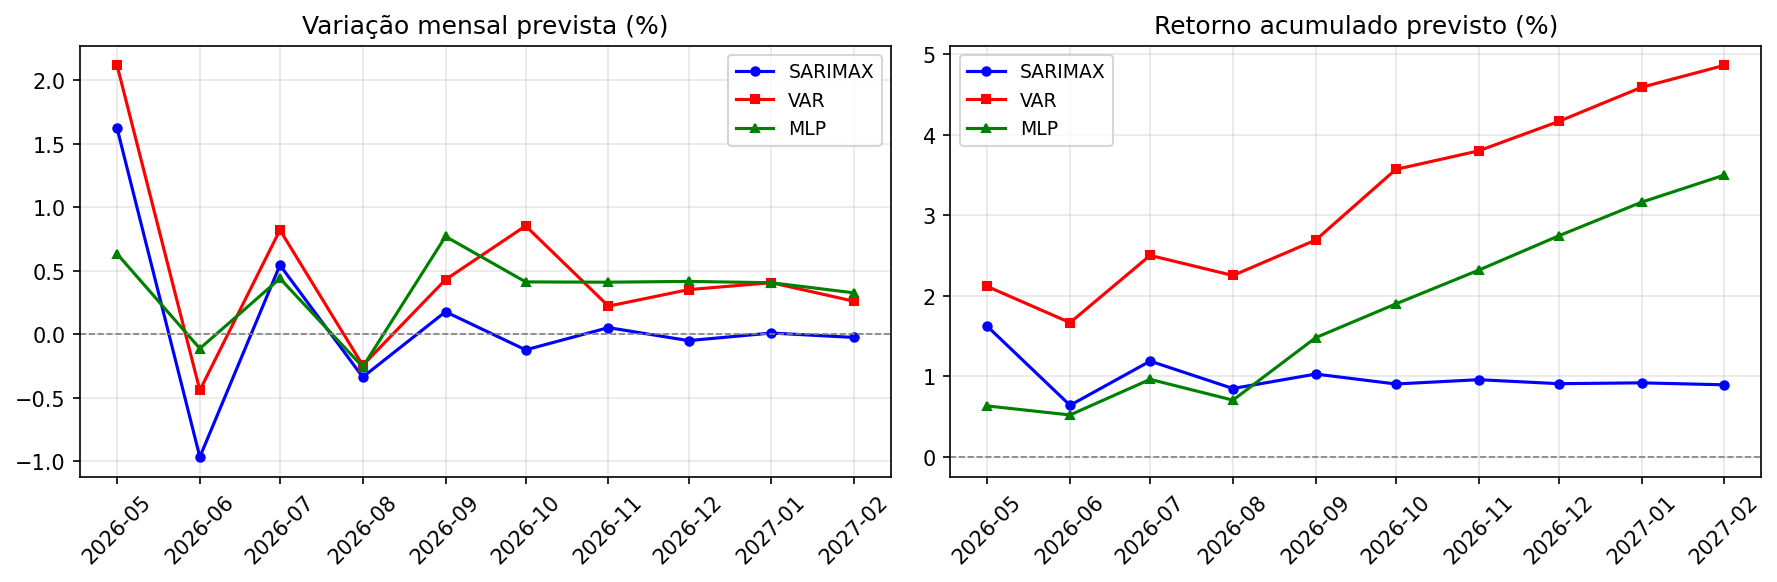
\includegraphics[width=\linewidth]{figures/forecast10.png}
\caption{Figura A2: previsão a 10~meses (maio de 2026 a fevereiro de 2027), variação mensal e retorno acumulado.}
\end{figure}

\end{document}
